\documentclass[11pt]{article}
\usepackage[T1]{fontenc}
\usepackage[a4paper,margin=0.9in]{geometry}
\usepackage{amsmath,amssymb,amsthm}
\usepackage{graphicx}
\usepackage{tikz}
\usepackage[hidelinks]{hyperref}
\usepackage{microtype}

\newtheorem{theorem}{Theorem}
\newtheorem{lemma}[theorem]{Lemma}
\newtheorem{proposition}[theorem]{Proposition}
\newtheorem{remark}[theorem]{Remark}
\newtheorem*{sourcequestion}{Source question (Remarks 4.5--4.6)}

\newcommand{\Lp}{L^p_h(M,N)}
\newcommand{\Dp}{D_p}

\setlength{\parindent}{0pt}
\setlength{\parskip}{0.55em}

\title{Separability Splits Length from Geodesic Structure\
in Nonlinear Lebesgue Spaces}
\author{Run \texttt{fa\_banach\_001} --- lane 16}
\date{11 August 2026}

\begin{document}
\maketitle

\begin{center}
\fbox{\parbox{0.91\textwidth}{
\textbf{Status: candidate partial result, likely valid.}
For the length-space conclusion in Proposition~4.4 of arXiv:2603.09459,
global separability of the complete target is unnecessary.  In contrast,
separability cannot be removed from the geodesic conclusion in general:
for every $p\in(1,\infty]$ there is a complete nonseparable geodesic target
$N$ for which the corresponding nonlinear $L^p$ space is not geodesic.
The possibility of dropping completeness remains open.
}}
\end{center}

\section{Source and question}

Guillaume S\'erieys, \emph{Nonlinear Lebesgue spaces: Curves and geometry},
arXiv:2603.09459 (2026), defines $L^p_h(M,N)$ using equivalence classes of
measurable maps with separable range and the metric
\[
 \Dp(f,g)=\left(\int_M d_N(f(x),g(x))^p\,d\mu(x)\right)^{1/p}
\]
for finite $p$, with the usual essential-supremum definition for $p=\infty$.
Proposition~4.4 proves that this space is a length (respectively geodesic)
space when $N$ is complete, separable, and length (respectively geodesic).

On arXiv PDF page~31 the source records the remaining issue~\cite{source}:

\begin{sourcequestion}
Can the completeness and separability assumptions on $N$ in
Proposition~4.4 be relaxed?
\end{sourcequestion}

\begin{center}

\includegraphics[width=0.96\textwidth]{figures/open_problem_crop.png}
\end{center}

The proof in the source uses completeness and separability to select a
measurable family of nearly minimizing pointwise curves.  The following
results show that the two conclusions behave differently.

\section{Results}

\begin{theorem}[Global separability is unnecessary for length spaces]
\label{th:length}
Let $(M,\Sigma,\mu)$ be any measure space, let $h\in L^0(M,N)$, and let
$p\in[1,\infty]$.  If $N$ is a complete length space, with no separability
assumption, then $L^p_h(M,N)$ is a length space.
\end{theorem}

\begin{theorem}[Separability cannot generally be dropped for geodesicity]
\label{th:counter}
For every $p\in(1,\infty]$ there exist a probability space
$(M,\Sigma,\mu)$, a complete nonseparable geodesic metric space $N$, and
$h\in L^0(M,N)$ such that $L^p_h(M,N)$ is not a geodesic space.
In the same examples it is a complete length space by
Theorem~\ref{th:length}.
\end{theorem}

Thus separability can be removed entirely from the length half of the source
proposition, but not from its geodesic half for $p>1$.  These statements do
not decide whether completeness can be dropped.

\section{Proof intuition}

The positive result uses the strong measurability built into the definition:
the base map and any two endpoints already have separable ranges.  A
countable approximate-midpoint closure of those ranges sits inside a closed,
separable, complete length subspace of $N$.  The source's measurable-selection
argument can then be run in that smaller target.

For the negative result, use an uncountable ladder.  The two rails are
separable, so the endpoint maps are admissible; the midpoint of each vertical
rung lies in an uncountable uniformly discrete set.  Strict convexity of the
scalar $L^p$ norm for $p>1$ forces any function-space midpoint to choose those
pointwise rung midpoints almost everywhere, making its range nonseparable.

\section{A separable length hull}

Call $z$ an $\varepsilon$-midpoint of $x,y$ if
\[
 \max\{d(x,z),d(z,y)\}\leq \tfrac12d(x,y)+\varepsilon.
\]

\begin{lemma}[Separable reduction]
\label{lem:hull}
If $X$ is a complete length space and $A\subset X$ is separable, then there
is a closed separable length subspace $Y\subset X$ containing $A$.
\end{lemma}

\begin{proof}
Choose a countable set $S_0$ dense in $A$.  Given a countable $S_n$, for
every $u,v\in S_n$ and every $k\geq1$, choose a $1/k$-midpoint
$m(u,v,k)$ in $X$, and put
\[
 S_{n+1}=S_n\cup\{m(u,v,k):u,v\in S_n,\ k\geq1\}.
\]
Such midpoints exist because a curve from $u$ to $v$ whose length is
arbitrarily close to $d(u,v)$ has a point arbitrarily close to half its
length.  Let
\[
 Y=\overline{\bigcup_{n\geq0}S_n}^{,X}.
\]
Then $Y$ is closed and separable, contains $A$, and is complete because $X$
is complete.

It remains to show that $Y$ is a length space.  Given $y,z\in Y$ and
$\varepsilon>0$, choose $u,v$ in the countable union at a common sufficiently
late stage with $d(y,u),d(z,v)<\delta$.  At the next stage choose
$m(u,v,k)$ with $1/k<\delta$.  The triangle inequality gives
\[
 \max\{d(y,m),d(m,z)\}
 \leq \tfrac12d(y,z)+3\delta.
\]
As $\delta$ is arbitrary, $Y$ has approximate midpoints with every positive
error.  The standard dyadic construction now gives, for every $\eta>0$, a
curve in $Y$ from $y$ to $z$ of length at most $d(y,z)+\eta$: recursively
insert approximate midpoints with summable errors, define the curve first on
dyadic times, and use completeness to extend it continuously.  Hence $Y$ is
a length space.
\end{proof}

\begin{proof}[Proof of Theorem~\ref{th:length}]
Choose separably valued representatives of $h,f,g$, where $f,g$ are arbitrary
elements of $L^p_h(M,N)$.  Their three ranges have separable union $A$.
Apply Lemma~\ref{lem:hull} to obtain a closed, separable, complete length
subspace $Y\subset N$ containing those ranges.

Now regard $h,f,g$ as $Y$-valued maps.  Proposition~4.4 of the source, applied
to $Y$, gives for every $\kappa>1$ an absolutely continuous curve $c$ from
$f$ to $g$ in $L^p_h(M,Y)$ with
\[
 L(c)\leq \kappa\Dp(f,g).
\]
The inclusion $Y\hookrightarrow N$ induces an isometric inclusion of the
corresponding nonlinear Lebesgue spaces, so $c$ is also an admissible curve in
$L^p_h(M,N)$.  Letting $\kappa\downarrow1$ proves that its intrinsic metric
equals $\Dp$.
\end{proof}

\section{The uncountable ladder counterexample}

Let $A=\{a_x:x\in[0,1]\}$ and $B=\{b_x:x\in[0,1]\}$ be two copies of the
unit interval, each with its usual length metric.  For every $x\in[0,1]$,
attach a distinct interval $E_x$ of length $2$, joining $a_x$ to $b_x$.
Give the resulting metric graph $N$ its intrinsic path metric.

\begin{center}
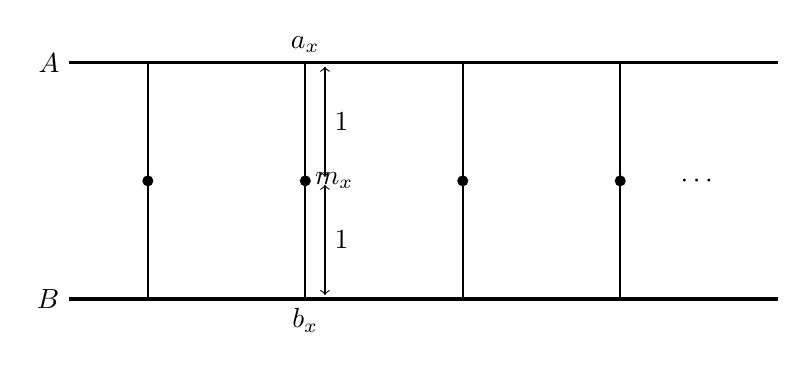
\begin{tikzpicture}[scale=1.0]
 \draw[very thick] (0,1.5)--(9,1.5);
 \draw[very thick] (0,-1.5)--(9,-1.5);
 \foreach \x/\lab in {1/{},3/{x},5/{y},7/{}} {
   \draw[thick] (\x,1.5)--(\x,-1.5);
   \fill (\x,0) circle (2pt);
 }
 \node[left] at (0,1.5) {$A$};
 \node[left] at (0,-1.5) {$B$};
 \node[above] at (3,1.5) {$a_x$};
 \node[below] at (3,-1.5) {$b_x$};
 \node[right] at (3,0) {$m_x$};
 \node at (8,0) {$\cdots$};
 \draw[<->] (3.25,1.45)--(3.25,0.05) node[midway,right] {$1$};
 \draw[<->] (3.25,-0.05)--(3.25,-1.45) node[midway,right] {$1$};
\end{tikzpicture}
\end{center}

\begin{lemma}[Geometry of the ladder]
\label{lem:ladder}
The space $N$ is complete and geodesic.  The edge $E_x$ is the unique
geodesic from $a_x$ to $b_x$.  If $m_x$ is its midpoint, then
$d_N(m_x,m_y)\geq2$ whenever $x\neq y$.
\end{lemma}

\begin{proof}
A shortest path can be reduced to one which uses at most one complete
vertical edge: any two unnecessary rail changes cost $4$ and can be replaced
by travel along a rail of length at most $1$.  Among the remaining candidates,
the possible crossing point belongs to the compact interval $[0,1]$ and the
path length depends continuously on it, so a minimum is attained.  Thus $N$
is geodesic.

For $a_x$ and $b_x$, the direct edge has length $2$.  A path crossing at
$z\neq x$ has length at least
$|x-z|+2+|z-x|>2$, proving uniqueness.  A path from $m_x$ to $m_y$ with
$x\neq y$ must first travel distance $1$ to an endpoint of $E_x$ and finally
distance $1$ from an endpoint of $E_y$, so the midpoints are $2$-separated.

Finally, let $(q_n)$ be Cauchy.  If it stays a fixed positive distance from
both rails, it must eventually lie in one vertical edge, because interiors of
distinct such edges are uniformly separated there.  Otherwise it approaches
one rail (it cannot alternate between the two, which are distance $2$ apart),
and its nearest rail coordinates form a Cauchy sequence in $[0,1]$.  In both
cases it converges in $N$, proving completeness.
\end{proof}

\begin{proof}[Proof of Theorem~\ref{th:counter}]
Take $M=[0,1]$ with Lebesgue measure and define
\[
 h(x)=f(x)=a_x,\qquad g(x)=b_x.
\]
The ranges of $f$ and $g$ are the two separable rails, so these maps are
admissible, and $\Dp(f,g)=2$ for every $p$.

Assume first that $1<p<\infty$ and that a constant-speed geodesic exists.
Let $w$ be its value at time $1/2$, represented by a separably valued map, and
write
\[
 r(x)=d_N(a_x,w(x)),\qquad s(x)=d_N(w(x),b_x).
\]
Then $r+s\geq2$ pointwise and
$\lVert r\rVert_p=\lVert s\rVert_p=1$.  Since the base measure has mass one,
\[
 2=\lVert2\rVert_p
 \leq\lVert r+s\rVert_p
 \leq\lVert r\rVert_p+\lVert s\rVert_p=2.
\]
Equality in Minkowski for nonnegative functions in $L^p$, $p>1$, forces
$r=s$ almost everywhere; their norms then give $r=s=1$ almost everywhere.
Together with $r+s=d(a_x,b_x)$, this says that $w(x)$ is the midpoint of a
geodesic from $a_x$ to $b_x$.  Lemma~\ref{lem:ladder} makes it the unique
point $m_x$.

For $p=\infty$, midpoint equality gives $r,s\leq1$ almost everywhere, while
$r+s\geq2$, so again $r=s=1$ and $w(x)=m_x$ almost everywhere.

Every full-measure subset of $[0,1]$ is uncountable, whereas every
$2$-separated subset of a separable metric space is countable.  Hence the
essential range $\{m_x\}$ of $w$ is not separable, contradicting the defining
requirement for membership in $L^p_h(M,N)$.  No geodesic exists.
\end{proof}

\begin{remark}[Why $p=1$ is different]
The counterexample is sharp with respect to the strict-convexity step.  For
$p=1$, define $c(t)(x)=b_x$ for $x\leq t$ and $c(t)(x)=a_x$ for $x>t$.
Then $D_1(c(s),c(t))=2|s-t|$, so $c$ is a geodesic whose value at every time
has separable range.  This agrees with the source's observation that
$L^1$-geodesics need not be pointwise geodesics.
\end{remark}

\section{Verification, limitations, and novelty}

The separable-hull proof was checked at the three points on which it depends:
the construction is countable; closure preserves completeness inside the
complete target; and the approximate-midpoint property passes from the
countable core to the closure with explicit $3\delta$ error.  The ladder was
checked directly for completeness, existence of minimizing paths, uniqueness
of the designated rungs, and uniform separation of their midpoints.  The
$L^p$ obstruction uses only equality in the scalar Minkowski inequality (or
the elementary essential-supremum inequality at $p=\infty$).

This is intentionally a partial answer.  It removes separability from the
length conclusion and disproves its general removal from the geodesic
conclusion for $p>1$, but it does not decide whether completeness can be
relaxed.  It also makes no negative claim for the geodesic conclusion at
$p=1$.

A bounded novelty search through 11 August 2026 checked the run registry,
exact source wording and title, approximate-midpoint separable reductions,
separable length subspaces, metric-valued $L^p$ geodesicity, nonseparable
targets, and measurable geodesic selection.  It found the source and general
selection-theorem literature but no matching theorem or ladder counterexample.
Novelty confidence is moderate and expert review is recommended, with special
attention to Lemma~\ref{lem:hull} and the metric-graph completeness argument.

\begin{thebibliography}{9}
\bibitem{source}
G. S\'erieys,
\emph{Nonlinear Lebesgue spaces: Curves and geometry},
arXiv:2603.09459, 2026.
\end{thebibliography}

\end{document}
